\begin{experiment}{Single \emph{exposer} versus \emph{exposer} ensemble comparison}{\small \sffamily\textbf{Description}

We are testing radius on range 0.01---0.3 using iris dataset, analyzing:

\begin{itemize}
\tightlist
	\item \texttt{2.3} --- \emph{Simple model}, a single exposer on lambda \textbf{[2, 3]}, grain \emph{90}, using \textbf{lone participation}.
	\item \texttt{ENS} --- \emph{Combined model}, an ensemble, using \textbf{brutal} approach, grain \emph{90}, dimensions \emph{[2]}, using \textbf{lone participation}.

\end{itemize}


\textbf{Results}

\centering
	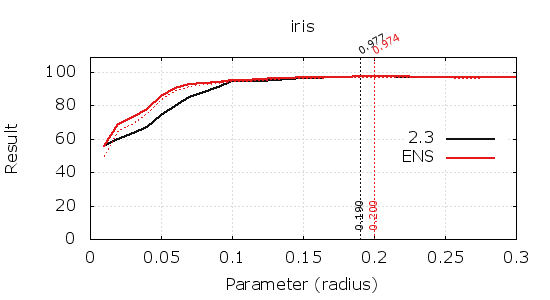
\includegraphics[width=.75\textwidth]{plots/experiment_3_iris.png}
	\captionof{figure}{Single \emph{exposer} versus \emph{exposer} ensemble comparison}
	\label{fig:experiment_3}
}\end{experiment}